\documentclass{../../fal_assignment}
\graphicspath{ {../../} }

\usepackage{enumitem}
\setlist{nosep} % Make enumerate / itemize lists more closely spaced
\usepackage[T1]{fontenc} % http://tex.stackexchange.com/a/17858
\usepackage{url}
\usepackage{todonotes}
\usepackage{float}

\title{Portfolio of Game Prototypes}
\author{Brian McDonald}
\module{GAM702}
\version{1.0}

\begin{document}

\maketitle

\section*{Introduction}

\begin{marginquote}
"It isn't enough to pick a path—you must go down it. By doing so, you see things you couldn't possibly see when you started out; you may not like what you see, some of it may be confusing, but at least you will have, as we like to say, 'explored the neighborhood.' The key point here is that even if you decide you're in the wrong place, there is still time to head toward the right place."
-- Ed Catmull, Creativity Inc.

\end{marginquote}
\marginpicture{flavour_pic}{
    \emph{Marvel's Spider-man: PS4}, early gameplay prototype showing web traversal mechanics.
}

For this assignment you will create \textbf{five} prototype games based on a series of provocations provided by the module tutor. In effect, you will be creating a small game prototype every two weeks. After the end of the two weeks, you will receive feedback from your Peers and the Module Tutors.

As a Game Designer it is up to you on what kind of game you create and what technology you will use to create the prototype. You can create a digital game, boardgame, cardgame, RPG Module or physical game. However, you will need to justify all your decisions in the Development Journal , see \textbf{Assignment 2}

For the final submission you have to select \textbf{three} prototypes that will go forward into your final summative submission.

For each part you must:
\begin{enumerate}[label=(\roman*)]
    \item \textbf{Read} the instructions in the worksheet or exercise sheet;
    \item \textbf{Complete} all of the problems presented;
    \item \textbf{Submit} your solution according to the instructions on the worksheet or exercise sheet, and by the deadline specified on the worksheet or exercise sheet.
\end{enumerate}

\subsection*{Assignment Setup} 

This assignment consists of \textbf{five formative submissions}, followed by a \textbf{single summative submission}.

The formative submissions consists of a single zip file, with the following folder structure. You can also find a template zip file on the Assignment Space in the Learning Space

\pagebreak
\textbf{Digital Game}

\begin{figure}[H]
	\begin{center}
		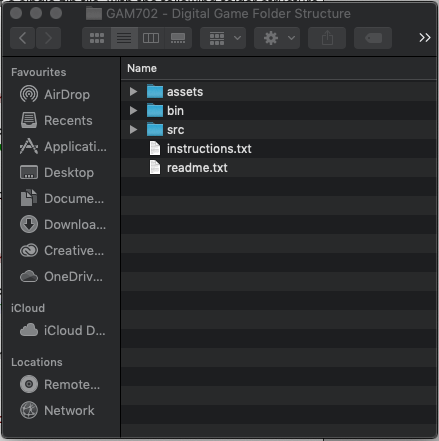
\includegraphics[height=0.4\textheight]{digital_games_folder_structure}
	\end{center}
	\caption{Recommended folder structure for formative submissions of Digital Games.}
	\label{fig:digital_game_folder_structure}
\end{figure}

\begin(enumerate)
	\item The \textbf{instructions.txt} should contain any controls and other information required to play
	\item The \textbf{readme.txt} should contain a description of the game and any references to resources used for the game. These resources include assets, reference materials, tutorials etc
	\item The \textbf{src} folder should contain the project files and source code for the game
	\item The \textbf{bin} folder should contain project combined executable
\end{enumerate}

\pagebreak
\textbf{Physical Game (including Boardgame, RPG and Folk Game)}



\begin{figure}[H]
	\begin{center}
		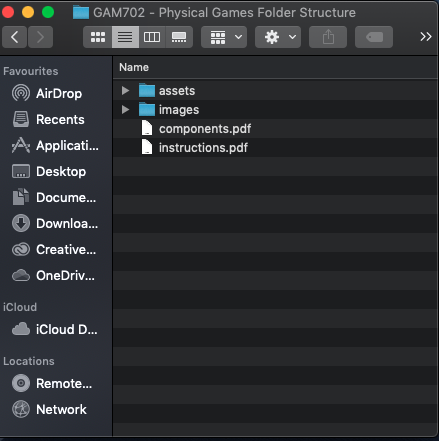
\includegraphics[height=0.4\textheight]{physical_games_folder_structure}
	\end{center}
	\caption{Recommended folder structure for formative submissions of Physical Games.}
	\label{fig:phyical_game_folder_structure}
\end{figure}

You will receive \textbf{feedback} after each formative submission.


At the end of the semester you will be required make a final summative submission of all five of your worksheet solutions \textbf{and} all five of your exercise sheet solutions.
Prepare a \textbf{single \texttt{.zip} file} containing your ten submissions \textbf{in ten separate folders}, and upload it to the appropriate submission area on LearningSpace. The folder structure within your zip file should resemble that shown in Figure~\ref{fig:final_games_folder_structure}.


\textbf{This final submission is subject to the usual university policies regarding late submission or non-submission,
as detailed in the course handbook ---
even if you have met all the formative deadlines for individual worksheets and exercise sheets,
failure to make a submission via LearningSpace by the summative deadline will be subject to penalties.}

\section*{Additional Guidance}



\section*{FAQ}

\begin{itemize}
	\item 	\textbf{What is the deadline for this assignment?} \\ 
    		Falmouth University policy states that summative deadlines must only be specified on the MyFalmouth system.
    		
	\item 	\textbf{What should I do to seek help?} \\ 
    		You can email your tutor for informal clarifications.  
    		
	\item 	\textbf{How will I receive feedback on my work?} \\ 
    		You will be given verbal feedback on your work during the session in which it is marked.
    		If you require more in-depth feedback or discussion, please book an appointment with your tutor.
    		
    	\item 	\textbf{Is this a mistake?} \\ 	
    		If you have discovered an issue with the brief itself, please inform the module tutor.
    		
\end{itemize}

\section*{Additional Resources}

\begin{itemize}
    \item F.\ Dunn and I.\ Parberry (2011). 3D Math Primer for Graphics and Game Development. CRC Press.
    \item E. Lengyel (2011). Foundations of Game Engine Development, Volume 1: Mathematics. Terathon Software LLC.
    \item T. Jenkyns and B. Stephenson (2012). Fundamentals of Discrete Math for Computer Science: A Problem-Solving Primer. Springer.
\end{itemize}

See also individual worksheets.

\newcommand{\wspercent}{12\%}
\newcommand{\espercent}{8\%}

\rubrichead{Each individual worksheet and exercise sheet is marked according to this rubric.}
\rubricfoot{Each worksheet is worth 15\% of the total marks for this assignment, and each exercise sheet worth 5\%.}
\begin{markingrubric}
	\firstcriterion{Basic competency threshold}{40\%}
		\grade\fail	A reasonable attempt at the worksheet or exercise sheet was not submitted by the formative deadline.
	\gradespan{5}{A reasonable attempt at the worksheet or exercise sheet was submitted by the formative deadline.
		\par		There is no evidence of academic misconduct.}
		
    \criterion{Other criteria}{60\%}
        \gradespan{6}{Please see individual worksheets and exercise sheets for marking criteria.}
\end{markingrubric}

\end{document}